\section{Experiments}
\label{sec:experiments}

\subsection{Protocols and Metrics}

We evaluate GDOR-SLAM on dynamic RGB-D sequences from TUM RGB-D~\cite{sturm2012benchmark} and Bonn RGB-D Dynamic~\cite{palazzolo2019bonn}.
The completed DYN-19 release is the primary evidence package.
Its main phase contains Semantic, MapMatched, and Full on ten claim-bearing sequences and seeds 0--2, for 90 runs; the denominator includes TUM sitting\_halfsphere.
The mechanism phase adds T+M, T+F+M, T+F+R+M, and Full-NoM on the same sequence/seed matrix, for 120 runs.
Here T, F, R, A, and M denote temporal-depth recovery, the residual-flow recovery veto, tracking-risk gating, adaptive FAST, and conservative persistent mapping weight.
The seven configurations form a predeclared \emph{ordered ablation}, not a factorial or fractional-factorial design.
The mapping phase evaluates Semantic, MapMatched, and Full over four scenes, three seeds, and online/GT-aligned render poses, for 72 cells.

Earlier frozen campaigns remain separate corroborating evidence.
\textbf{DYN-15} contains Semantic, GDOR, and Strict with three seeds on TUM walking\_xyz and all six Bonn dynamic sequences, for 63 runs.
\textbf{DYN-18} uses the unchanged configurations on the four TUM sequences named in the DyPho-SLAM tracking table, for 36 cells after one exact Semantic sitting seed-0 repair.
\textbf{DYN-17} is the three-sequence predecessor of the DYN-19 map-matched control.
\textbf{DYN-16} is a seed-0 common-view mapping diagnostic on TUM walking\_xyz and Bonn crowd and is retained only as a limited preservation diagnostic.

All tracking runs process the full association file and retain invalid intervals in the all-input-frame trajectory.
We report SE(3)-aligned ATE RMSE, one-frame translational RPE RMSE, failure rate, and end-to-end wall time.
Mapping uses common non-keyframe manifests and reports full/static PSNR and SSIM; LPIPS is unavailable in the DYN-19 release and is not imputed.
Occluded-background completeness and ghost-risk values are reported only as proxy diagnostics.

The benchmark harness records the source snapshot, executable and library hashes, detector-engine hash, configuration hash, association and ground-truth hashes, sequence, seed, command line, and output identity.
DYN-19 binds every result to source commit \texttt{14c6b2c}, frozen plan hashes, per-frame logs, run summaries, and recovered-support overlap certificates.
The public release contains trajectories, masks, maps, renders, per-frame logs, certificates, plans, summaries, and SHA-256 manifests.

\subsection{Tracking Accuracy and Frozen Generalization}

\begin{table*}[t]
\centering
\caption{Tracking evidence and external-report positioning. Panel A contains local same-source results; every reported mean improvement is accompanied by its failure case, median, and win/tie/loss count. Panel B copies paper-reported ATE values for context. Rows marked $\dagger$ use different run counts, estimators, implementations, or protocols and are not pooled with local results or used for a protocol-matched ranking.}
\label{tab:main-tracking}
\footnotesize
\resizebox{\linewidth}{!}{%
\begin{tabular}{lllrrrrll}
\toprule
Evidence & Scope & Cells represented & Semantic & GDOR & Strict & GDOR reduction & Failure/median context & W/T/L \\
\midrule
DYN-15 & Bonn6 mean & 54 & 12.837 & \textbf{4.079} & 8.526 & 68.2\% & crowd2 52.184$\rightarrow$3.226; med. 4.988$\rightarrow$3.577 & 6/0/0 \\
DYN-15 & All7 mean & 63 & 11.331 & \textbf{3.798} & 7.611 & 66.5\% & crowd2 52.184$\rightarrow$3.226; med. 4.278$\rightarrow$3.261 & 7/0/0 \\
\midrule
DYN-18 & TUM4 mean & 36 & 9.746 & 3.415 & \textbf{3.345} & 65.0\% & sitting 32.374$\rightarrow$7.354; med. paired gain 0.209 & 9/0/3 \\
\bottomrule
\end{tabular}
}

\vspace{0.6ex}
\resizebox{\linewidth}{!}{%
\begin{tabular}{llrrrrrl}
\toprule
Panel B method & Source & walking\_xyz & walking\_half & walking\_static & sitting\_half & Avg. & Reported statistic \\
\midrule
DynaSLAM$^\dagger$ & \cite{bescos2018dynaslam}, Table II & 1.500 & 2.500 & 0.600 & 1.700 & 1.575 & ten-run median ATE \\
DG-SLAM$^\dagger$ & \cite{xu2024dgslam}, Table 2 & 1.600 & -- & 0.600 & -- & -- & reported subset \\
DyPho-SLAM$^\dagger$ & \cite{liu2025dyphoslam}, Table I & 1.600 & 2.600 & 0.600 & 1.600 & 1.600 & ATE with reported Std. \\
GDOR DYN-18 (local) & This work & 2.119 & 3.344 & 0.843 & 7.354 & 3.415 & three-seed means \\
\bottomrule
\end{tabular}
}
\end{table*}

In DYN-15, GDOR reduces the All7 mean ATE from 11.331 cm to 3.798 cm, shifts the sequence-median ATE from 4.278 cm to 3.261 cm, and wins every declared sequence mean relative to Semantic (7/0/0 wins/ties/losses).
The largest rescue is Bonn crowd2 at 52.184 cm to 3.226 cm.
DYN-18 yields a 9/0/3 paired-cell record and a 0.209 cm median paired gain, but its mean change from 9.746 cm to 3.415 cm is driven mainly by sitting\_halfsphere at 32.374 cm to 7.354 cm.
The two-sided exact sign test is not significant ($p=0.146$), so DYN-18 is interpreted as conditional failure-regime rescue plus near-identity behavior elsewhere.
Panel B makes the published tracking gap visible without treating unlike protocols as paired observations.
The local GDOR row is not below the reported DyPho-SLAM row on any of the four sequence means; DG-SLAM reports only two of these four sequences in its own TUM table.

\begin{figure*}[t]
  \centering
  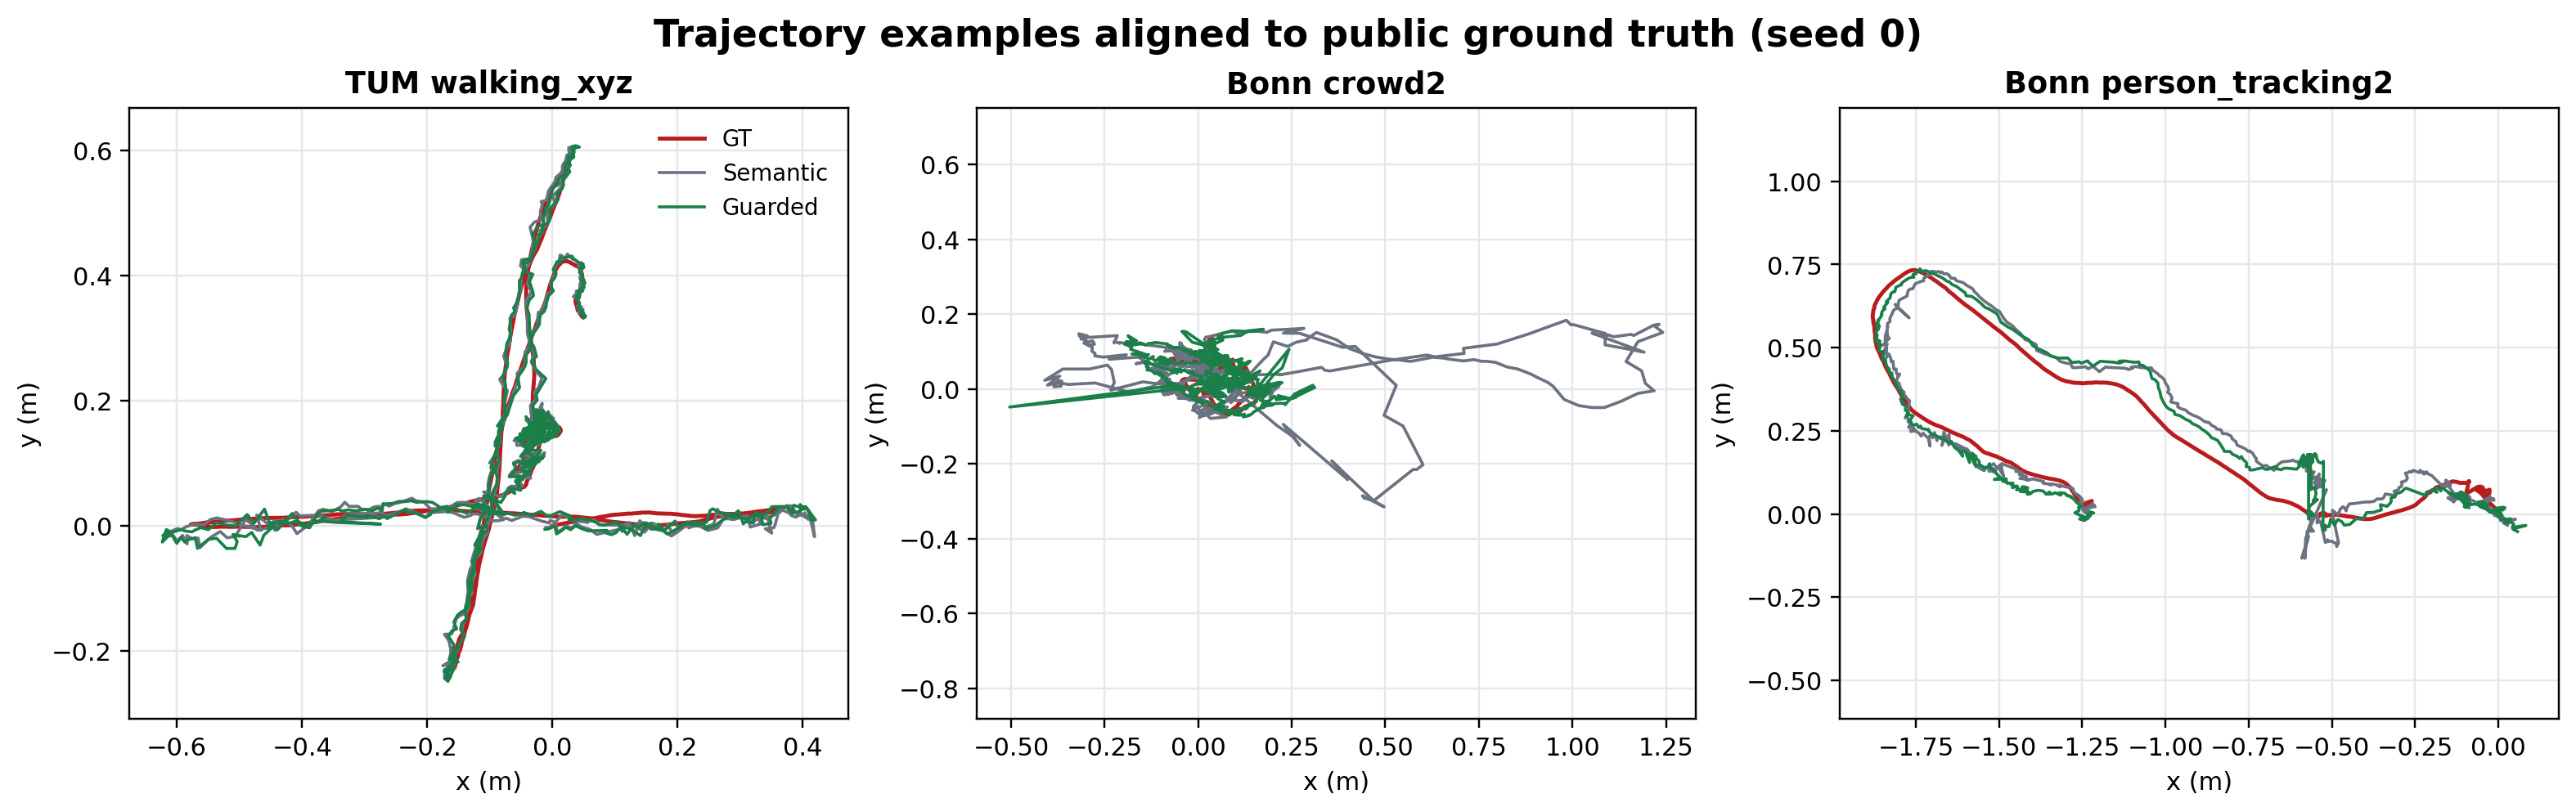
\includegraphics[width=\linewidth]{figures/fig3_trajectory_examples.png}
  \caption{Seed-0 trajectory examples aligned to public ground truth from the DYN-15 experiment family. The plots are qualitative diagnostics; Table~\ref{tab:main-tracking} uses all input frames and three-seed means.}
  \label{fig:trajectories}
\end{figure*}

\subsection{DYN-19 Main Extension and Ordered Ablation}

\begin{table*}[t]
\centering
\caption{Completed DYN-19 tracking results. Panel A reports the two claim-bearing Full comparisons over 30 paired cells; sequence W/T/L is computed after averaging the three seeds. Panel B is an ordered ablation. Its adjacent contrasts do not identify independent component effects or interactions. Positive adjacent medians mean the current row has lower paired-cell ATE than the preceding row.}
\label{tab:dyn19}
\footnotesize
\resizebox{\linewidth}{!}{%
\begin{tabular}{lrrrrllll}
\toprule
Panel A comparison & Cells & Baseline & Full & Reduction & Failure case & Paired median gain & Cell W/T/L & Sequence W/T/L \\
\midrule
Semantic $\rightarrow$ Full & 30 & 10.119 & \textbf{4.930} & 51.3\% & crowd2 42.500$\rightarrow$11.080 & 0.213 cm & 19/0/11 & 7/0/3 \\
MapMatched $\rightarrow$ Full & 30 & 7.392 & \textbf{4.930} & 33.3\% & sitting 36.775$\rightarrow$4.864 & 0.016 cm & 16/0/14 & 4/0/6 \\
\bottomrule
\end{tabular}
}

\vspace{0.5ex}
\resizebox{\linewidth}{!}{%
\begin{tabular}{lccccc rrll}
\toprule
Panel B configuration & T & F & R & A & M & Mean ATE & Median ATE & Adjacent median; W/T/L & Route certificate \\
\midrule
Semantic & 0 & 0 & 0 & 0 & 0 & 10.119 & 4.348 & -- & 30 vacuous \\
MapMatched & 0 & 0 & 0 & 0 & 1 & 7.392 & 3.824 & $+0.211$; 18/0/12 & 30 vacuous \\
T+M & 1 & 0 & 0 & 0 & 1 & \textbf{3.859} & 3.489 & $+0.023$; 17/0/13 & 30 pass \\
T+F+M & 1 & 1 & 0 & 0 & 1 & 6.377 & 3.748 & $-0.020$; 15/0/15 & 30 pass \\
T+F+R+M & 1 & 1 & 1 & 0 & 1 & 4.907 & 3.721 & $-0.024$; 14/0/16 & 30 pass \\
Full: T+F+R+A+M & 1 & 1 & 1 & 1 & 1 & 4.930 & 3.640 & $-0.006$; 15/0/15 & 30 pass \\
Full-NoM & 1 & 1 & 1 & 1 & 0 & 4.060 & 3.627 & $+0.025$; 18/0/12 & 30 fail (expected) \\
\bottomrule
\end{tabular}
}
\end{table*}

Table~\ref{tab:dyn19} broadens the matched control to all ten claim-bearing sequences.
Relative to Semantic, Full lowers the 30-cell mean from 10.119 cm to 4.930 cm, with a 0.213 cm paired-cell median gain and a 19/0/11 cell record; the largest failure-case rescue is Bonn crowd2 at 42.500 cm to 11.080 cm.
Relative to MapMatched, Full lowers the mean from 7.392 cm to 4.930 cm, but the paired median is only 0.016 cm, the cell record is 16/0/14, and Full wins only four of ten sequence means.
That aggregate is dominated by sitting\_halfsphere, where MapMatched reaches 36.775 cm and Full reaches 4.864 cm.
The supported interpretation is therefore severe-failure rescue rather than uniform improvement.

Panel B is deliberately non-monotonic.
T+M has the lowest overall mean, the flow-veto row is worse in mean despite a 6/0/4 sequence-mean record against T+M, and adding adaptive FAST changes the mean only from 4.907 cm to 4.930 cm with a 15/0/15 paired-cell split.
These adjacent bundle contrasts motivate the modules operationally but do not estimate independent causal effects.
Full-NoM obtains lower tracking ATE than Full, yet all 30 of its route certificates fail by construction because recovered support is admitted to persistent mapping; tracking accuracy alone is therefore insufficient evidence for the routing safety claim.

\begin{figure*}[t]
  \centering
  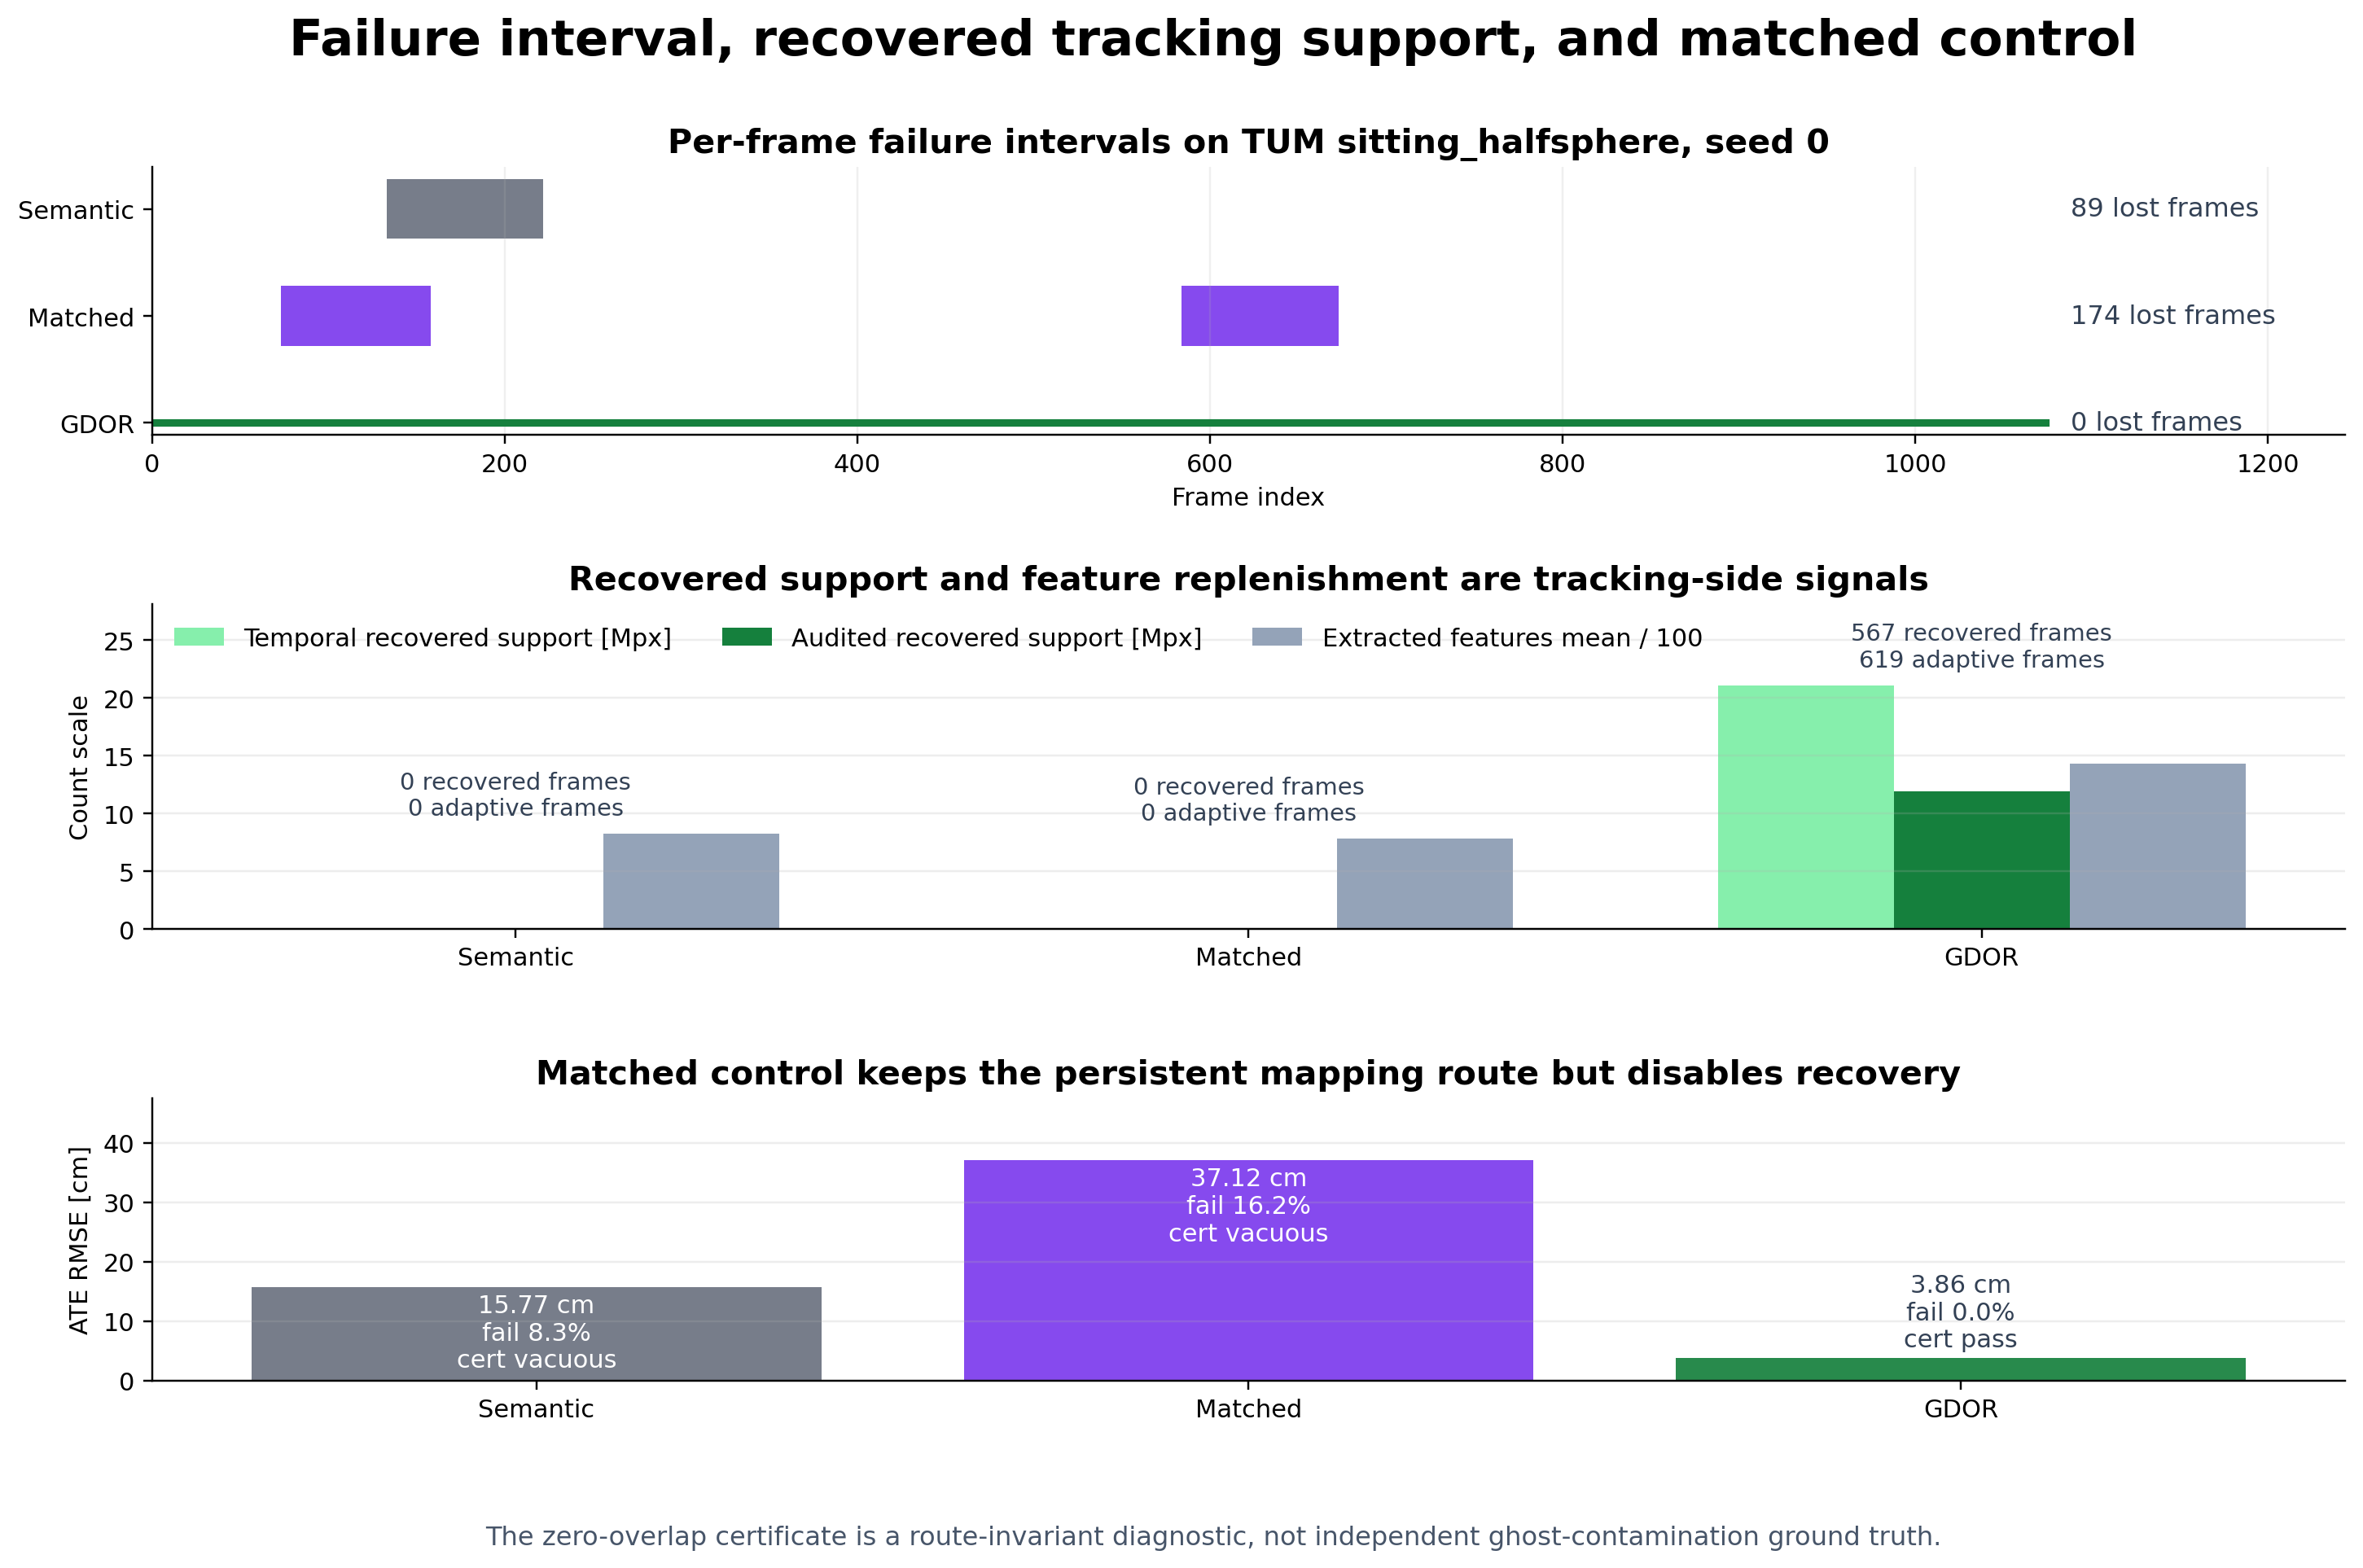
\includegraphics[width=\linewidth]{figures/fig5_failure_recovery_control.png}
  \caption{Representative DYN-19 route diagnostic on TUM sitting\_halfsphere, seed 0. Top: failure intervals from per-frame tracking logs. Middle: recovered support and adaptive feature activity are observed only in Full; these are tracking-side signals. Bottom: MapMatched shares the persistent mapping weight but disables qualified tracking recovery. The Full certificate records 567 recovered-support frames, 11.918M audited pixels, and no observed overlap with map-admissible support in this episode; this is a route diagnostic, not independent ghost-contamination truth.}
  \label{fig:failure-recovery-control}
\end{figure*}

\subsection{Safety, Route Certificate, and Mapping Diagnostic}

\begin{table*}[t]
\centering
\caption{Safety, efficiency, and mapping evidence. Panel A reports the DYN-15 All7 mean. Panel B represents all 72 DYN-19 mapping cells: 12 sequence/seed cells per method in each pose mode. Completeness and ghost-risk columns are occluded-background proxies, not independent ground truth. Panel C records published external mapping evidence under each source's native metric; heterogeneous metrics are not ranked against one another.}
\label{tab:safety-efficiency}
\footnotesize
\begin{tabular}{llrrrrr}
\toprule
Panel & Method & ATE [cm] $\downarrow$ & t-RPE [cm] $\downarrow$ & Failure [\%] $\downarrow$ & Time [s/run] $\downarrow$ & Map support [\%] \\
\midrule
A: DYN-15 All7 & Semantic & 11.331 & 4.277 & 0.785 & \textbf{32.46} & 100.00 \\
& GDOR & \textbf{3.798} & \textbf{3.945} & \textbf{0.144} & 49.84 & 63.31 \\
& Strict & 7.611 & 4.556 & 0.318 & 63.61 & 63.31 \\
\midrule
\multicolumn{7}{c}{}\\[-1.8ex]
\toprule
Panel B pose & Method & Static PSNR $\uparrow$ & Static SSIM $\uparrow$ & Proxy completeness $\uparrow$ & Proxy ghost risk $\downarrow$ & Cells \\
\midrule
Online & Semantic & 18.866 & 0.695 & 0.582 & \textbf{0.181} & 12 \\
& MapMatched & 18.990 & 0.700 & 0.579 & 0.184 & 12 \\
& Full & \textbf{19.763} & \textbf{0.728} & \textbf{0.582} & 0.188 & 12 \\
GT-aligned & Semantic & 12.082 & 0.492 & 0.402 & 0.351 & 12 \\
& MapMatched & 12.442 & 0.503 & 0.428 & 0.329 & 12 \\
& Full & \textbf{13.491} & \textbf{0.533} & \textbf{0.440} & \textbf{0.312} & 12 \\
\bottomrule
\end{tabular}

\vspace{0.6ex}
\resizebox{\linewidth}{!}{%
\begin{tabular}{lllll}
\toprule
Panel C method & Source/data & Evaluation object & Reported mapping result & Comparability to DYN-19 \\
\midrule
DG-SLAM$^\dagger$ & \cite{xu2024dgslam}, BONN5 & Mesh vs. GT point cloud & Acc. 8.06 cm; Comp. 15.46 cm; Comp.$@5$ cm 43.67\% & Different output metric and protocol \\
DyPho-SLAM$^\dagger$ & \cite{liu2025dyphoslam}, TUM/BONN & Novel-view render & Qualitative Fig.~4; no PSNR/SSIM/LPIPS table & No numeric mapping row \\
DynaSLAM$^\dagger$ & \cite{bescos2018dynaslam}, TUM & Static map and RGB-D inpainting & Qualitative maps/inpainting; no map-quality metric & No numeric mapping row \\
GDOR DYN-19 (local) & TUM/BONN4, 12 online cells & Held-out static-region render & PSNR 19.763 dB; SSIM 0.728 & Local diagnostic, not geometry GT \\
\bottomrule
\end{tabular}
}
\end{table*}

GDOR lowers the DYN-15 All7 failure rate but increases wall time from 32.46 s/run to 49.84 s/run.
Map support is the mean fraction of pixels satisfying $W_t^{\mathrm{map}}\ge0.5$, not a quality score.
The archived DYN-15--18 rejection counters show active static-weight gates, but only DYN-19 contains the direct overlap certificate from Eq.~\eqref{eq:leak-audit}.

Across the 12 online mapping cells per method, Full raises static PSNR from 18.866 dB for Semantic to 19.763 dB: the mean gain is 0.896 dB, the paired median gain is 0.544 dB, and the record is 9/0/3; the lowest-Semantic failure cell is sitting\_halfsphere seed 1 at 14.275 dB versus 16.551 dB for Full.
Against MapMatched, the corresponding mean is 18.990 dB to 19.763 dB, with a 0.515 dB paired median gain and an 11/0/1 record; its lowest cell is the same sitting sequence/seed at 14.009 dB versus 16.551 dB.
The GT-aligned rows are still end-to-end diagnostics because online poses constructed each map.
The proxy columns are non-monotonic in online mode and do not support a true ghost-contamination or complete-background claim.

Panel C separates external-paper availability from metric comparability.
DG-SLAM reports quantitative BONN geometry against a ground-truth point cloud, whereas DYN-19 reports held-out static-region image fidelity; neither value can be converted into the other.
The DyPho-SLAM and DynaSLAM papers provide qualitative mapping or inpainting examples but no PSNR/SSIM/LPIPS or geometric map-quality table that can be copied into a homogeneous DYN-19 ranking.

All 30 Full cells pass the recovered-support certificate, covering 3,751 recovered-support frames and 79,498,476 audited pixels with zero observed overlap against map-admissible support.
The T+M, T+F+M, and T+F+R+M rows also have 30 passing certificates each.
The 30 expected Full-NoM failures contain 90,790,462 overlapping pixels, providing a negative counterfactual that distinguishes the route invariant from a vacuous rejection counter.

The DYN-16 figure is retained as historical evidence only.
It uses two scenes, one seed, fixed static masks, and no independent ghost/completeness truth, so it remains a limited preservation diagnostic rather than a zero-ghost, zero-contamination, or broad mapping-superiority result.

\begin{figure*}[t]
  \centering
  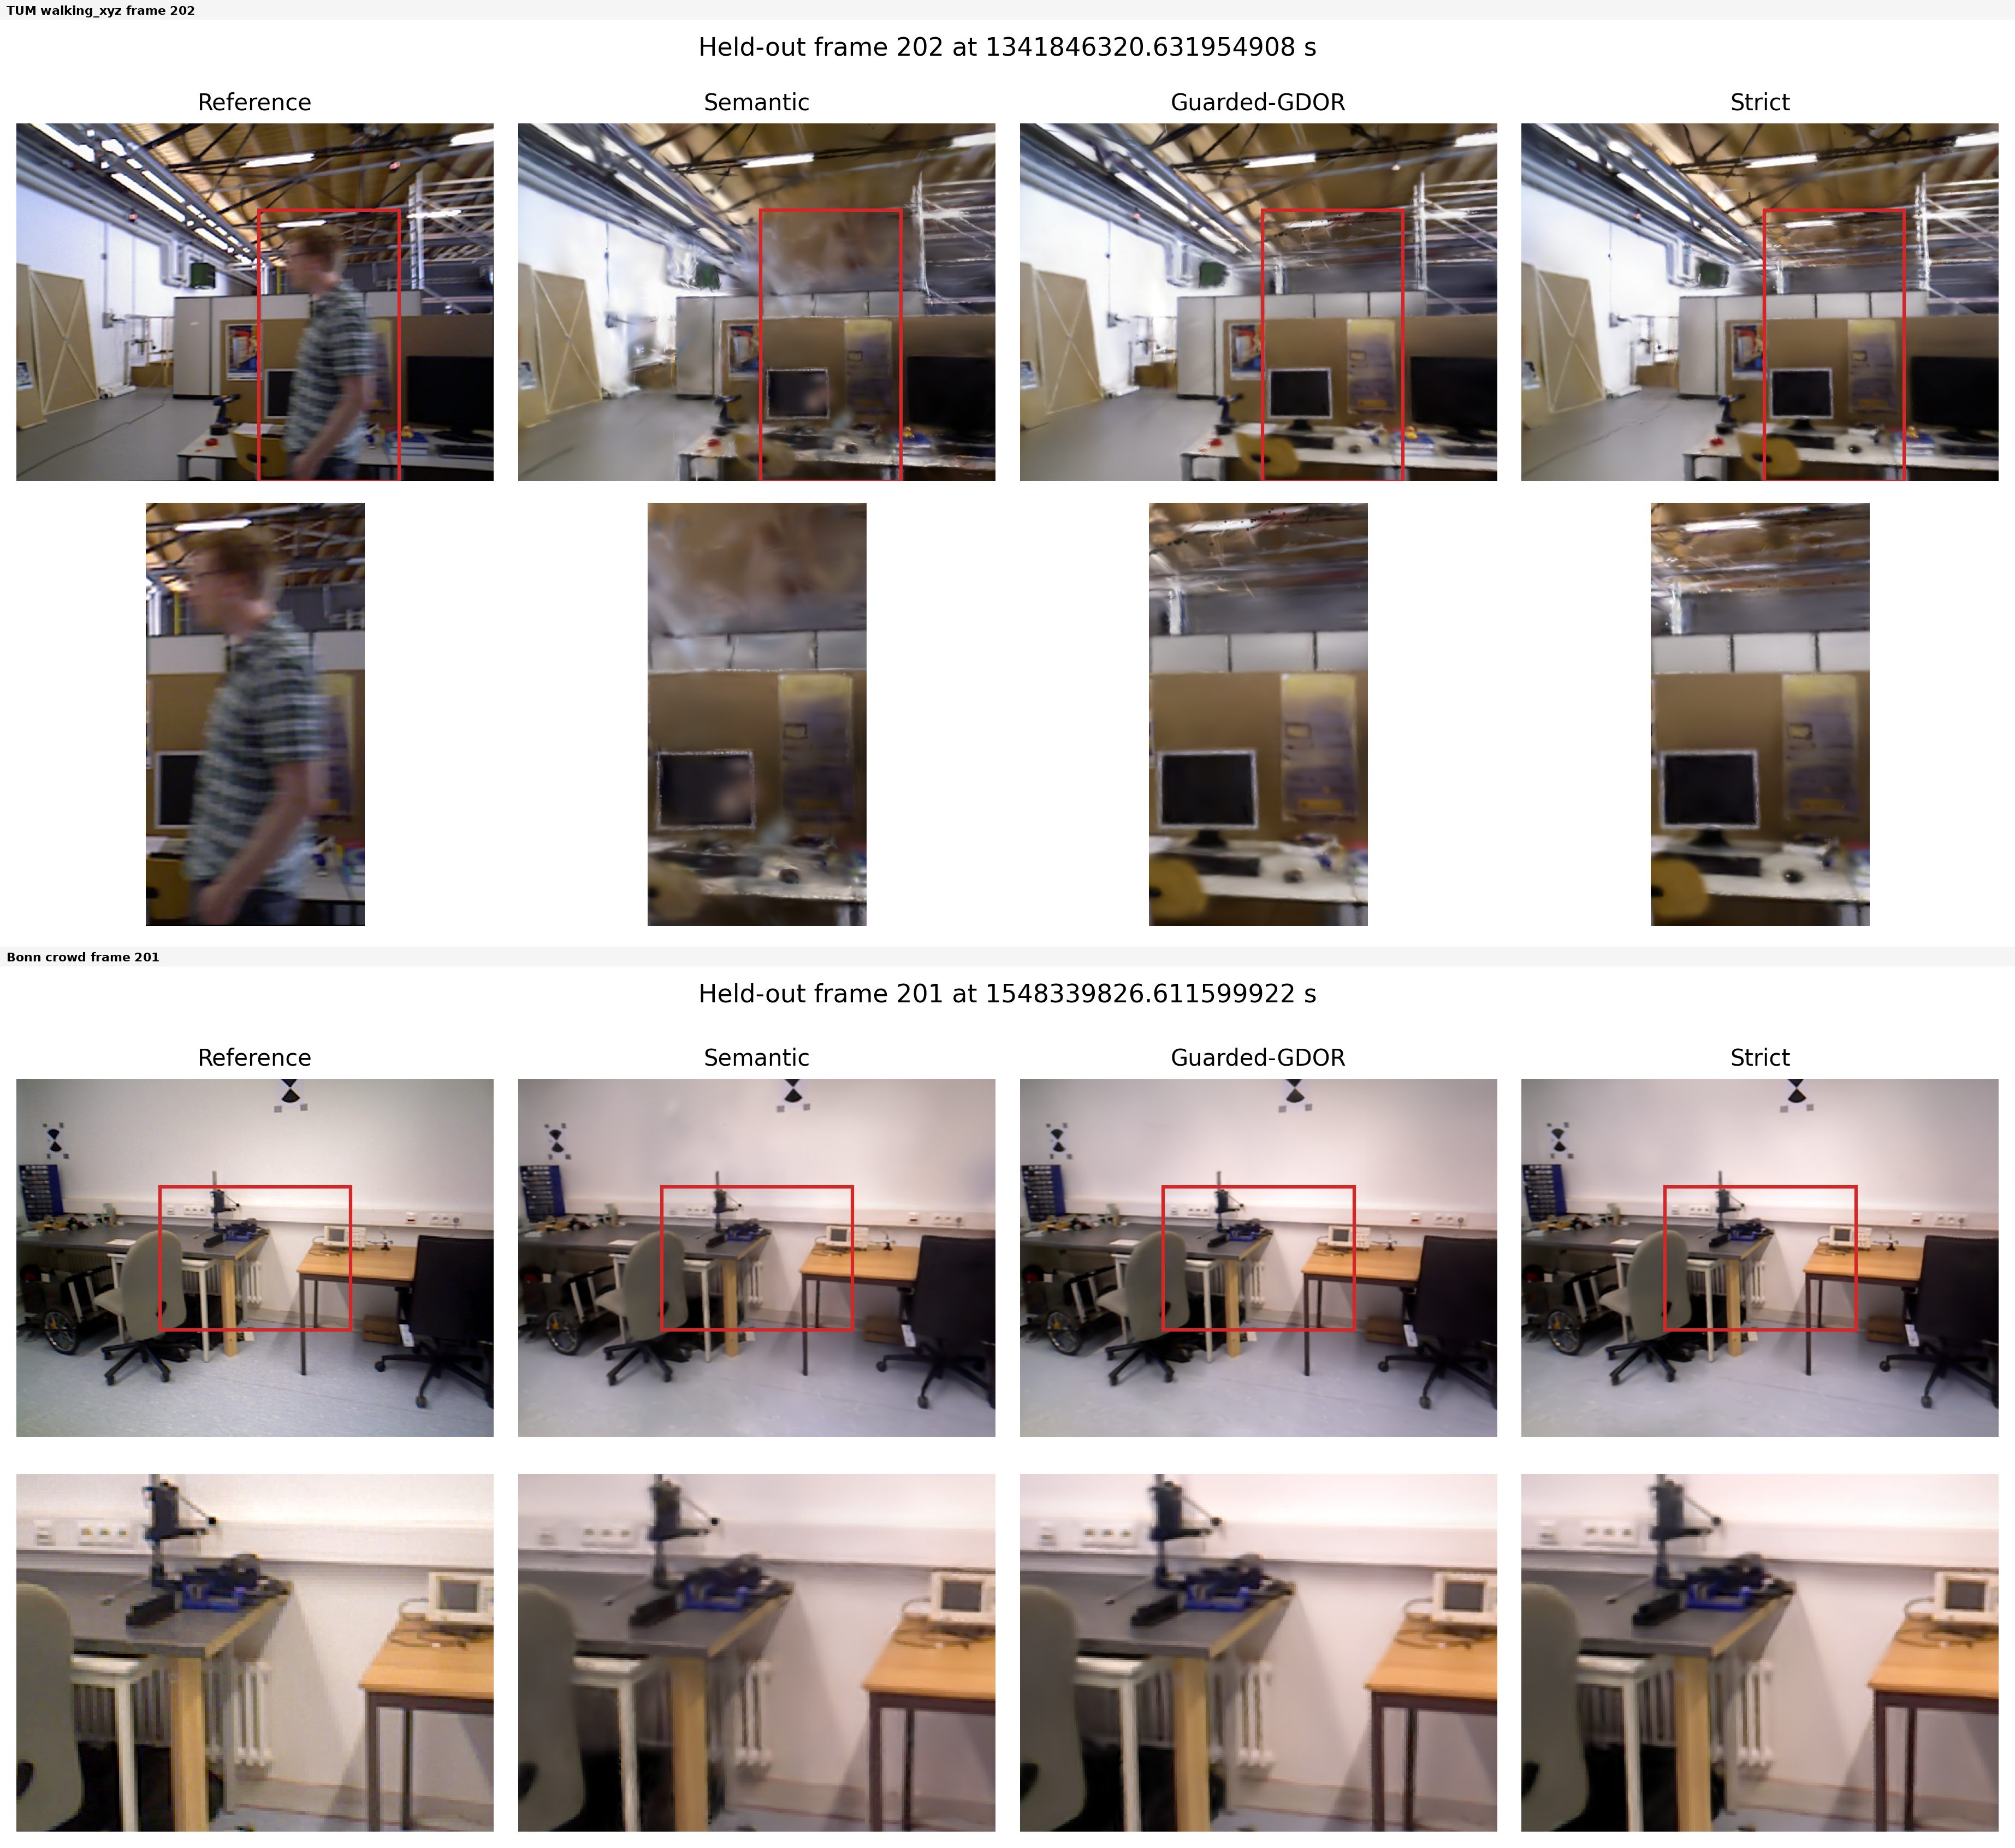
\includegraphics[width=\linewidth]{figures/fig4_commonview_mapping_audit.png}
  \caption{DYN-16 common-view online mapping diagnostic. Each row uses the same held-out frame, fixed static-region mask, and final-map render for Semantic, GDOR, and Strict. This historical single-seed view is retained as a limited preservation diagnostic; the quantitative multi-seed mapping result is in Table~\ref{tab:safety-efficiency}.}
  \label{fig:mapping}
\end{figure*}

\subsection{External Positioning and Limitations}

Published DG-SLAM, DyPho-SLAM, and DynaSLAM values are included in Tables~\ref{tab:main-tracking} and~\ref{tab:safety-efficiency} as explicitly marked external reports rather than protocol-matched DYN-19 rows.
The audited DG-SLAM runner uses ground-truth poses inside its shipped Gaussian mapping path, while the audited DynaSLAM source lacks an accepted ten-sequence TUM/Bonn execution path.
Both therefore remain ineligible as local protocol-matched rows until online-pose, association, mask-provenance, artifact, and no-failure eligibility gates pass.
The DyPho-SLAM paper reports 1.6, 2.6, 0.6, and 1.6 cm on the four corresponding TUM sequences; GDOR is not below those external values in DYN-18, and protocol differences prevent a direct ranking.

DYN-19 closes the earlier multi-seed and common-manifest mapping gap, but not the independent-truth gap.
Its occluded-background proxy is constructed from the same RGB-D sequences and frozen semantic masks.
Blind manual labels or external revealed-background truth with agreement/adjudication and provenance certificates are still required before claiming measured ghost contamination or complete-background recovery.
